\newpage
\subsection{Rigid body \& IMU kinematics}
\begin{wrapfigure}[5]{r}{0.3\columnwidth}
    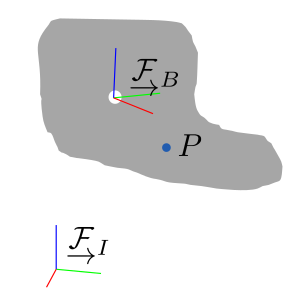
\includegraphics[width=0.3\columnwidth]{assets/rigid-body-6d.png}
\end{wrapfigure}
\bi{Velocity} ${_I}\vec{v}_{IB} = {_I}\dot{\vec{t}}_B$

\bi{Rot. Velocity} ${_I}\vec{\omega}_{IB} = \dot{\alpha} \cdot {_I}\vec{n}$

\bi{Velocity point $P$} ${_B}\vec{v}_{IP} = {_B}\vec{v}_{IB} + {_B}\vec{\omega}_{IB} \times {_B}\vec{t}_{P}$

\bi{Rotation Matrices}
\begin{itemize}
    \item For left pertubing\\
          $\mat{\dot{R}}_{IB} = [{_I} \omega_{IB}]^\times \mat{R}_{IB}$
    \item For right pertubing
          $\mat{\dot{R}}_{IB} = \mat{R}_{IB} [{_I} \omega_{IB}]^\times$
    \item Constant angular velocity ($\exp{[\Delta \vec{\alpha}]^\times} = \delta \mat{R}(\Delta \vec{\alpha})$)\\
          $\mat{R}_{IB}(t + \Delta t) = \exp{[\Delta \vec{\alpha}]^\times} \mat{R}_{IB}(t) \quad \vec{\alpha} = {_I}\vec{\omega}_{IB} \delta t$
\end{itemize}

\bi{Quaternions}
\begin{itemize}
    \item For left pertubing
          $\vec{\dot{q}}_{IB} =
              \frac{1}{2}
              {\scriptsize
                  \begin{bmatrix}
                      {_I}\vec{\omega}_{IB} \\
                      0
                  \end{bmatrix}
              }
              \otimes \vec{q}_{IB}$
    \item For right pertubing
          $\vec{\dot{q}}_{IB} =
              \frac{1}{2} \vec{q}_{IB} \otimes
              {\scriptsize
                  \begin{bmatrix}
                      {_B}\vec{\omega}_{IB} \\
                      0
                  \end{bmatrix}
              }$
\end{itemize}

\bi{IMU} (Outputs {\color{blue} ${_S}\vec{\tilde{a}}$} (accel.), {\color{red} ${_S}\vec{\tilde{\omega}}$} (rot. accel.))\\
${_W}\vec{\dot{t}}_S = {_W} \vec{v}$;
$\quad \displaystyle \vec{\dot{q}}_{WS} = \frac{1}{2} \vec{q}_{WS} \otimes
    {\scriptsize
        \begin{bmatrix}
            {\color{red}{_S}\vec{\tilde{\omega}}} {\color{gray} + \vec{w}_g - \vec{b}_g} \\
            0
        \end{bmatrix}
    }$

${_W}\vec{\dot{v}} = \mat{R}_{WS}\; ({\color{blue}{_S}\vec{\tilde{a}}} {\color{gray} + \vec{w}_a - \vec{b}_a}) + {_W}\vec{g}$
where {\color{gray} gray parts} only IRL (in theor. models, leave out), with $\vec{\dot{b}}_g = \vec{w}_{b_g}$ and $\vec{\dot{b}}_a = \vec{w}_{b_a}$

\bi{IMU Sensor Model}: $\vec{\tilde{z}} = \vec{b}_C + s\mat{M}\vec{z} + \vec{b} + \vec{n} + \vec{o}$
where bias $\vec{b}$ and scale $s$ often modelled time-varying $\dot{b}(t) = \sigma_C n(t)$.
$\vec{b}_C$ const. calib; $\mat{M}$ Misalignment; $\vec{n}$ noise; $\vec{o}$ other infl.
